% Digital Logic Report Template
% Created: 2020-01-10, John Miller

%==========================================================
%=========== Document Setup  ==============================

% Formatting defined by class file
\documentclass[11pt]{article}

% ---- Document formatting ----
\usepackage[margin=1in]{geometry}	% Narrower margins
\usepackage{booktabs}				% Nice formatting of tables
\usepackage{graphicx}				% Ability to include graphics

%\setlength\parindent{0pt}	% Do not indent first line of paragraphs 
\usepackage[parfill]{parskip}		% Line space b/w paragraphs
%	parfill option prevents last line of pgrph from being fully justified

% Parskip package adds too much space around titles, fix with this
\RequirePackage{titlesec}
\titlespacing\section{0pt}{8pt plus 4pt minus 2pt}{3pt plus 2pt minus 2pt}
\titlespacing\subsection{0pt}{4pt plus 4pt minus 2pt}{-2pt plus 2pt minus 2pt}
\titlespacing\subsubsection{0pt}{2pt plus 4pt minus 2pt}{-6pt plus 2pt minus 2pt}

% ---- Hyperlinks ----
\usepackage[colorlinks=true,urlcolor=blue]{hyperref}	% For URL's. Automatically links internal references.

% ---- Code listings ----
\usepackage{listings} 					% Nice code layout and inclusion
\usepackage[usenames,dvipsnames]{xcolor}	% Colors (needs to be defined before using colors)

% Define custom colors for listings
\definecolor{listinggray}{gray}{0.98}		% Listings background color
\definecolor{rulegray}{gray}{0.7}			% Listings rule/frame color

% Style for Verilog
\lstdefinestyle{Verilog}{
	language=Verilog,					% Verilog
	backgroundcolor=\color{listinggray},	% light gray background
	rulecolor=\color{blue}, 			% blue frame lines
	frame=tb,							% lines above & below
	linewidth=\columnwidth, 			% set line width
	basicstyle=\small\ttfamily,	% basic font style that is used for the code	
	breaklines=true, 					% allow breaking across columns/pages
	tabsize=3,							% set tab size
	commentstyle=\color{gray},	% comments in italic 
	stringstyle=\upshape,				% strings are printed in normal font
	showspaces=false,					% don't underscore spaces
}

% How to use: \Verilog[listing_options]{file}
\newcommand{\Verilog}[2][]{%
	\lstinputlisting[style=Verilog,#1]{#2}
}




%======================================================
%=========== Body  ====================================
\begin{document}

\title{ELC 2137 Lab \07: Binary Coded Decimal }
\author{Spencer Stinson}
\maketitle
\section*{Summary}
In this lab experiment, we learned how to use the double dabble method to convert from hex to BCD values. This method can be implemented by using multiple instances of adders. To finish this lab, we had to implement this 11 bit BCD decoder, as well as our 7 segment design fro mthe previous lab. 

\section*{Code}\\

\Verilog[caption= add3 code ]{C:/Users/spencer_stinson1/Documents/GitHub/Lab07/Lab07/Lab07.srcs/sources_1/new/add3.sv}
\Verilog[caption= double dabble 6 bit code]{C:/Users/spencer_stinson1/Documents/GitHub/Lab07/Lab07/Lab07.srcs/sources_1/new/dd6b.sv}
\Verilog[caption= double dabble 11 bit code ]{C:/Users/spencer_stinson1/Documents/GitHub/Lab07/Lab07/Lab07.srcs/sources_1/new/dd11b.sv}
\Verilog[caption=7 segment BCD code]{C:/Users/spencer_stinson1/Documents/GitHub/Lab07/Lab07/Lab07.srcs/sources_1/new/sseg1_bcd.sv}
\Verilog[caption= testbench for add3 code]{C:/Users/spencer_stinson1/Documents/GitHub/Lab07/Lab07/Lab07.srcs/sim_1/new/add3_testbench.sv}
\Verilog[caption= testbench for double dabble 6 bit code]{C:/Users/spencer_stinson1/Documents/GitHub/Lab07/Lab07/Lab07.srcs/sim_2/new/dd6b_testbench_.sv}
\Verilog[caption = testbench for double dabble 11 bit]{C:/Users/spencer_stinson1/Documents/GitHub/Lab07/Lab07/Lab07.srcs/sim_3/new/dd11b_testbench.sv}
\section*{Results}

In this section, put your simulation waveforms, results tables, pictures of hardware, and any other required items.
\begin{figure}
	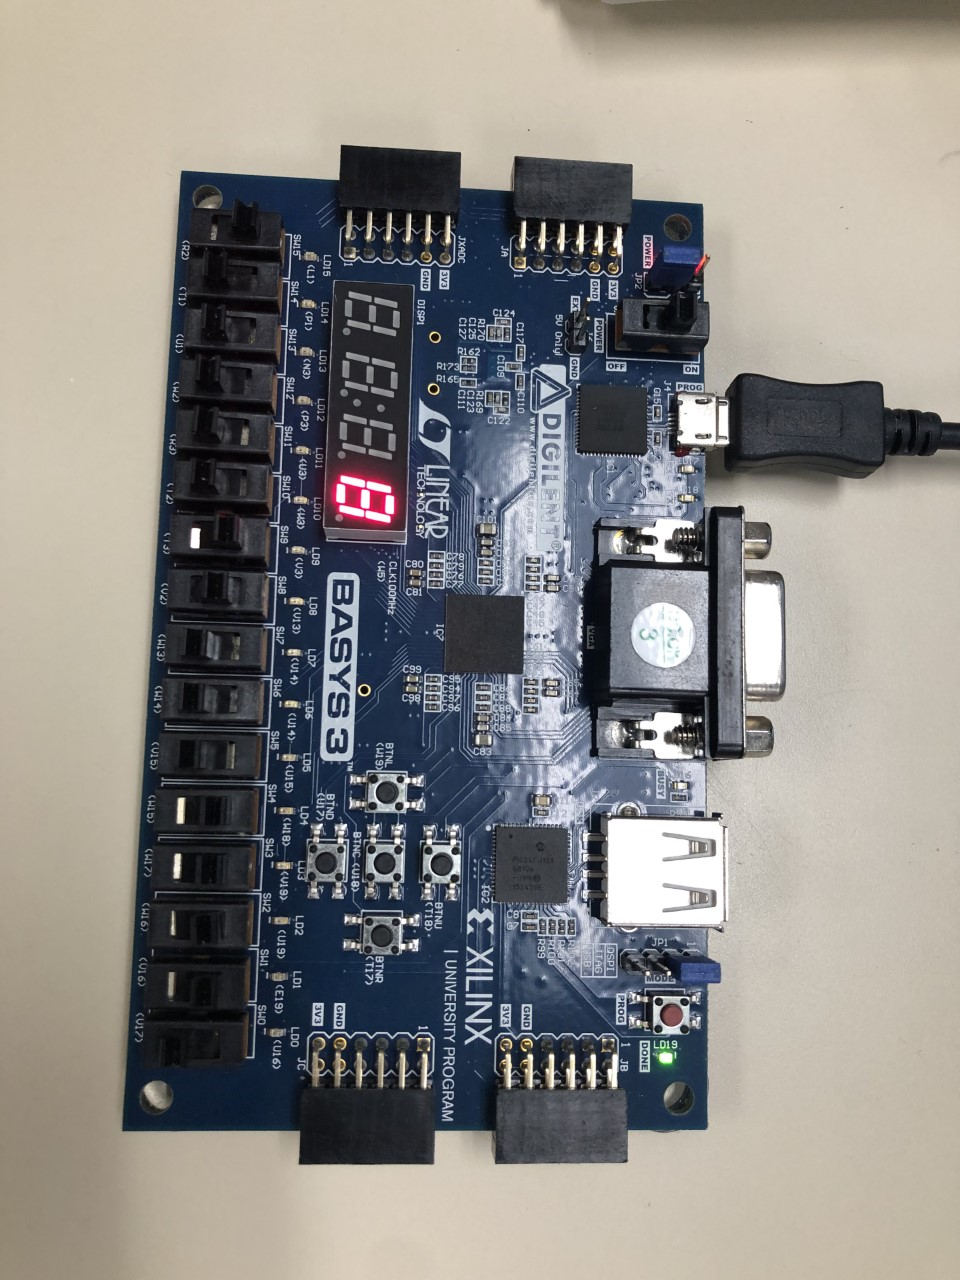
\includegraphics[width= \textwidth]{basys1.png}
	\caption{Basys board running 7 segment on first display }\label{fig:Basys1}
\end{figure}
\begin{figure}
	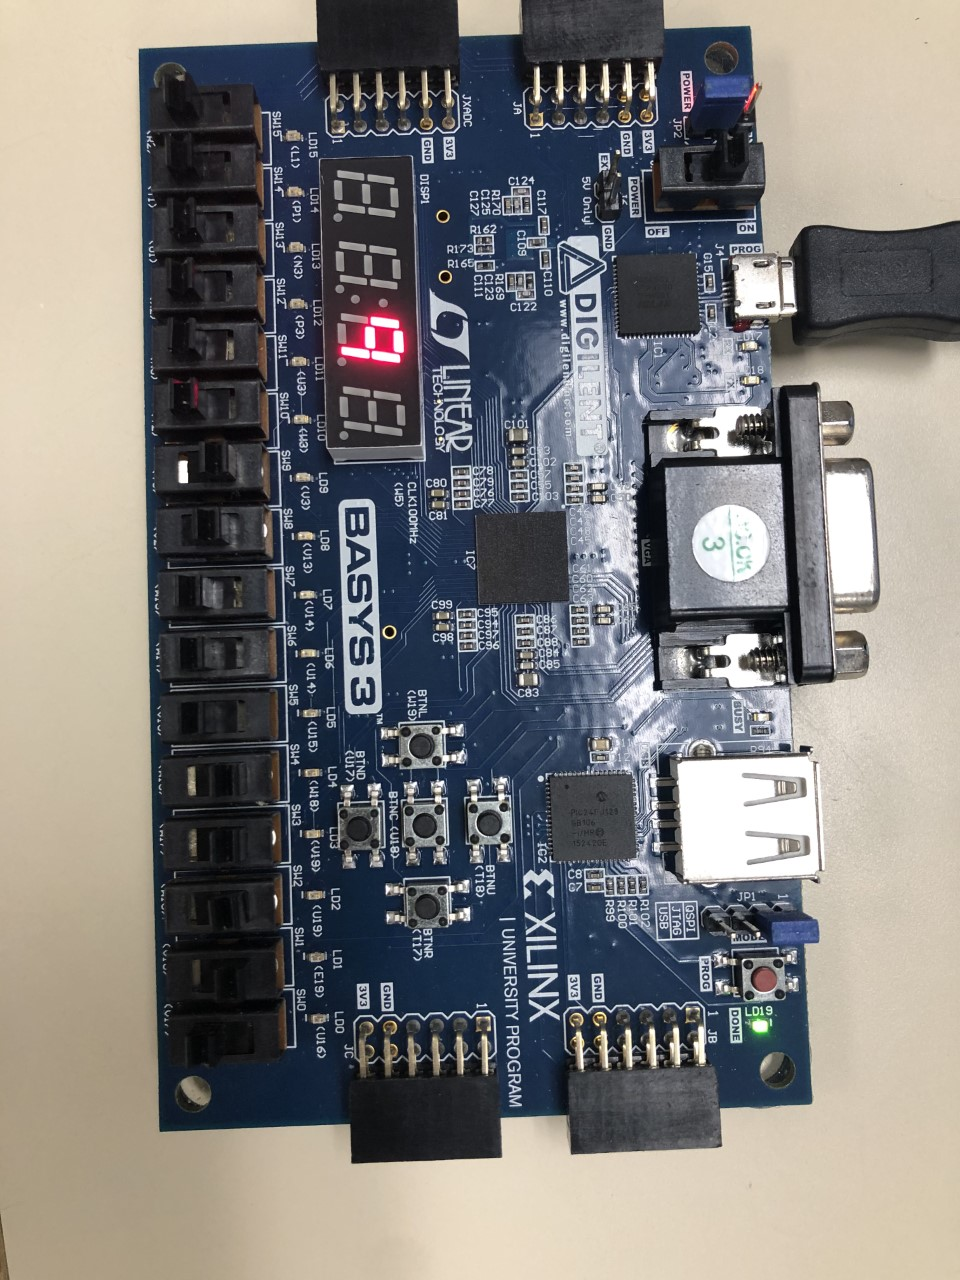
\includegraphics[width= \textwidth]{basys2.png}
	\caption{Basys board running 7 segment on second display }\label{fig:Basys2}
\end{figure}
\begin{figure}
	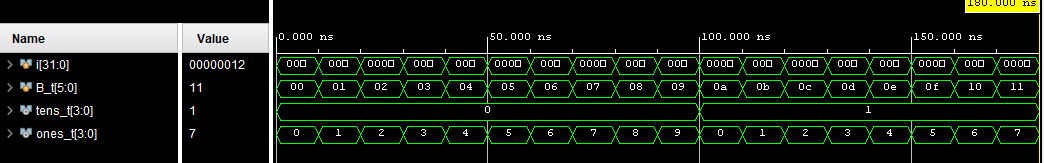
\includegraphics[width= \textwidth]{dd6bsc.png}
	\caption{waveform for 6-bit}\label{fig:dd6b}
\end{figure}
\begin{figure}
	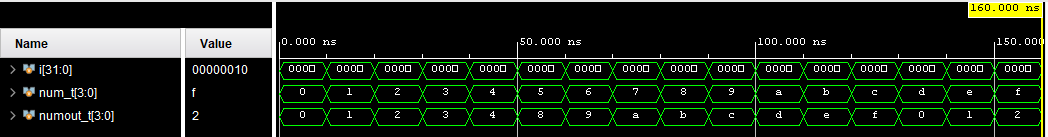
\includegraphics[width= \textwidth]{add3sc.png}
	\caption{waveform for add3}\label{fig:add3}
\end{figure}
\begin{figure}
	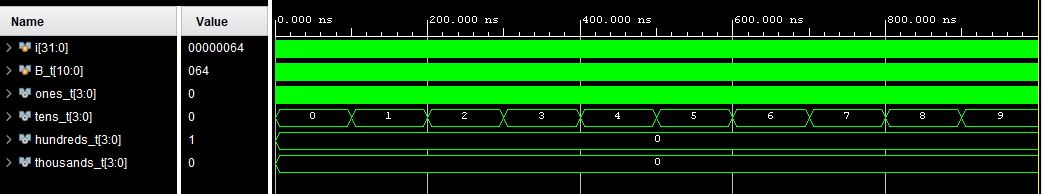
\includegraphics[width= \textwidth]{dd11bsc.png}
	\caption{waveform for 11-bit}\label{fig:dd11b}
\end{figure}
\begin{figure}
	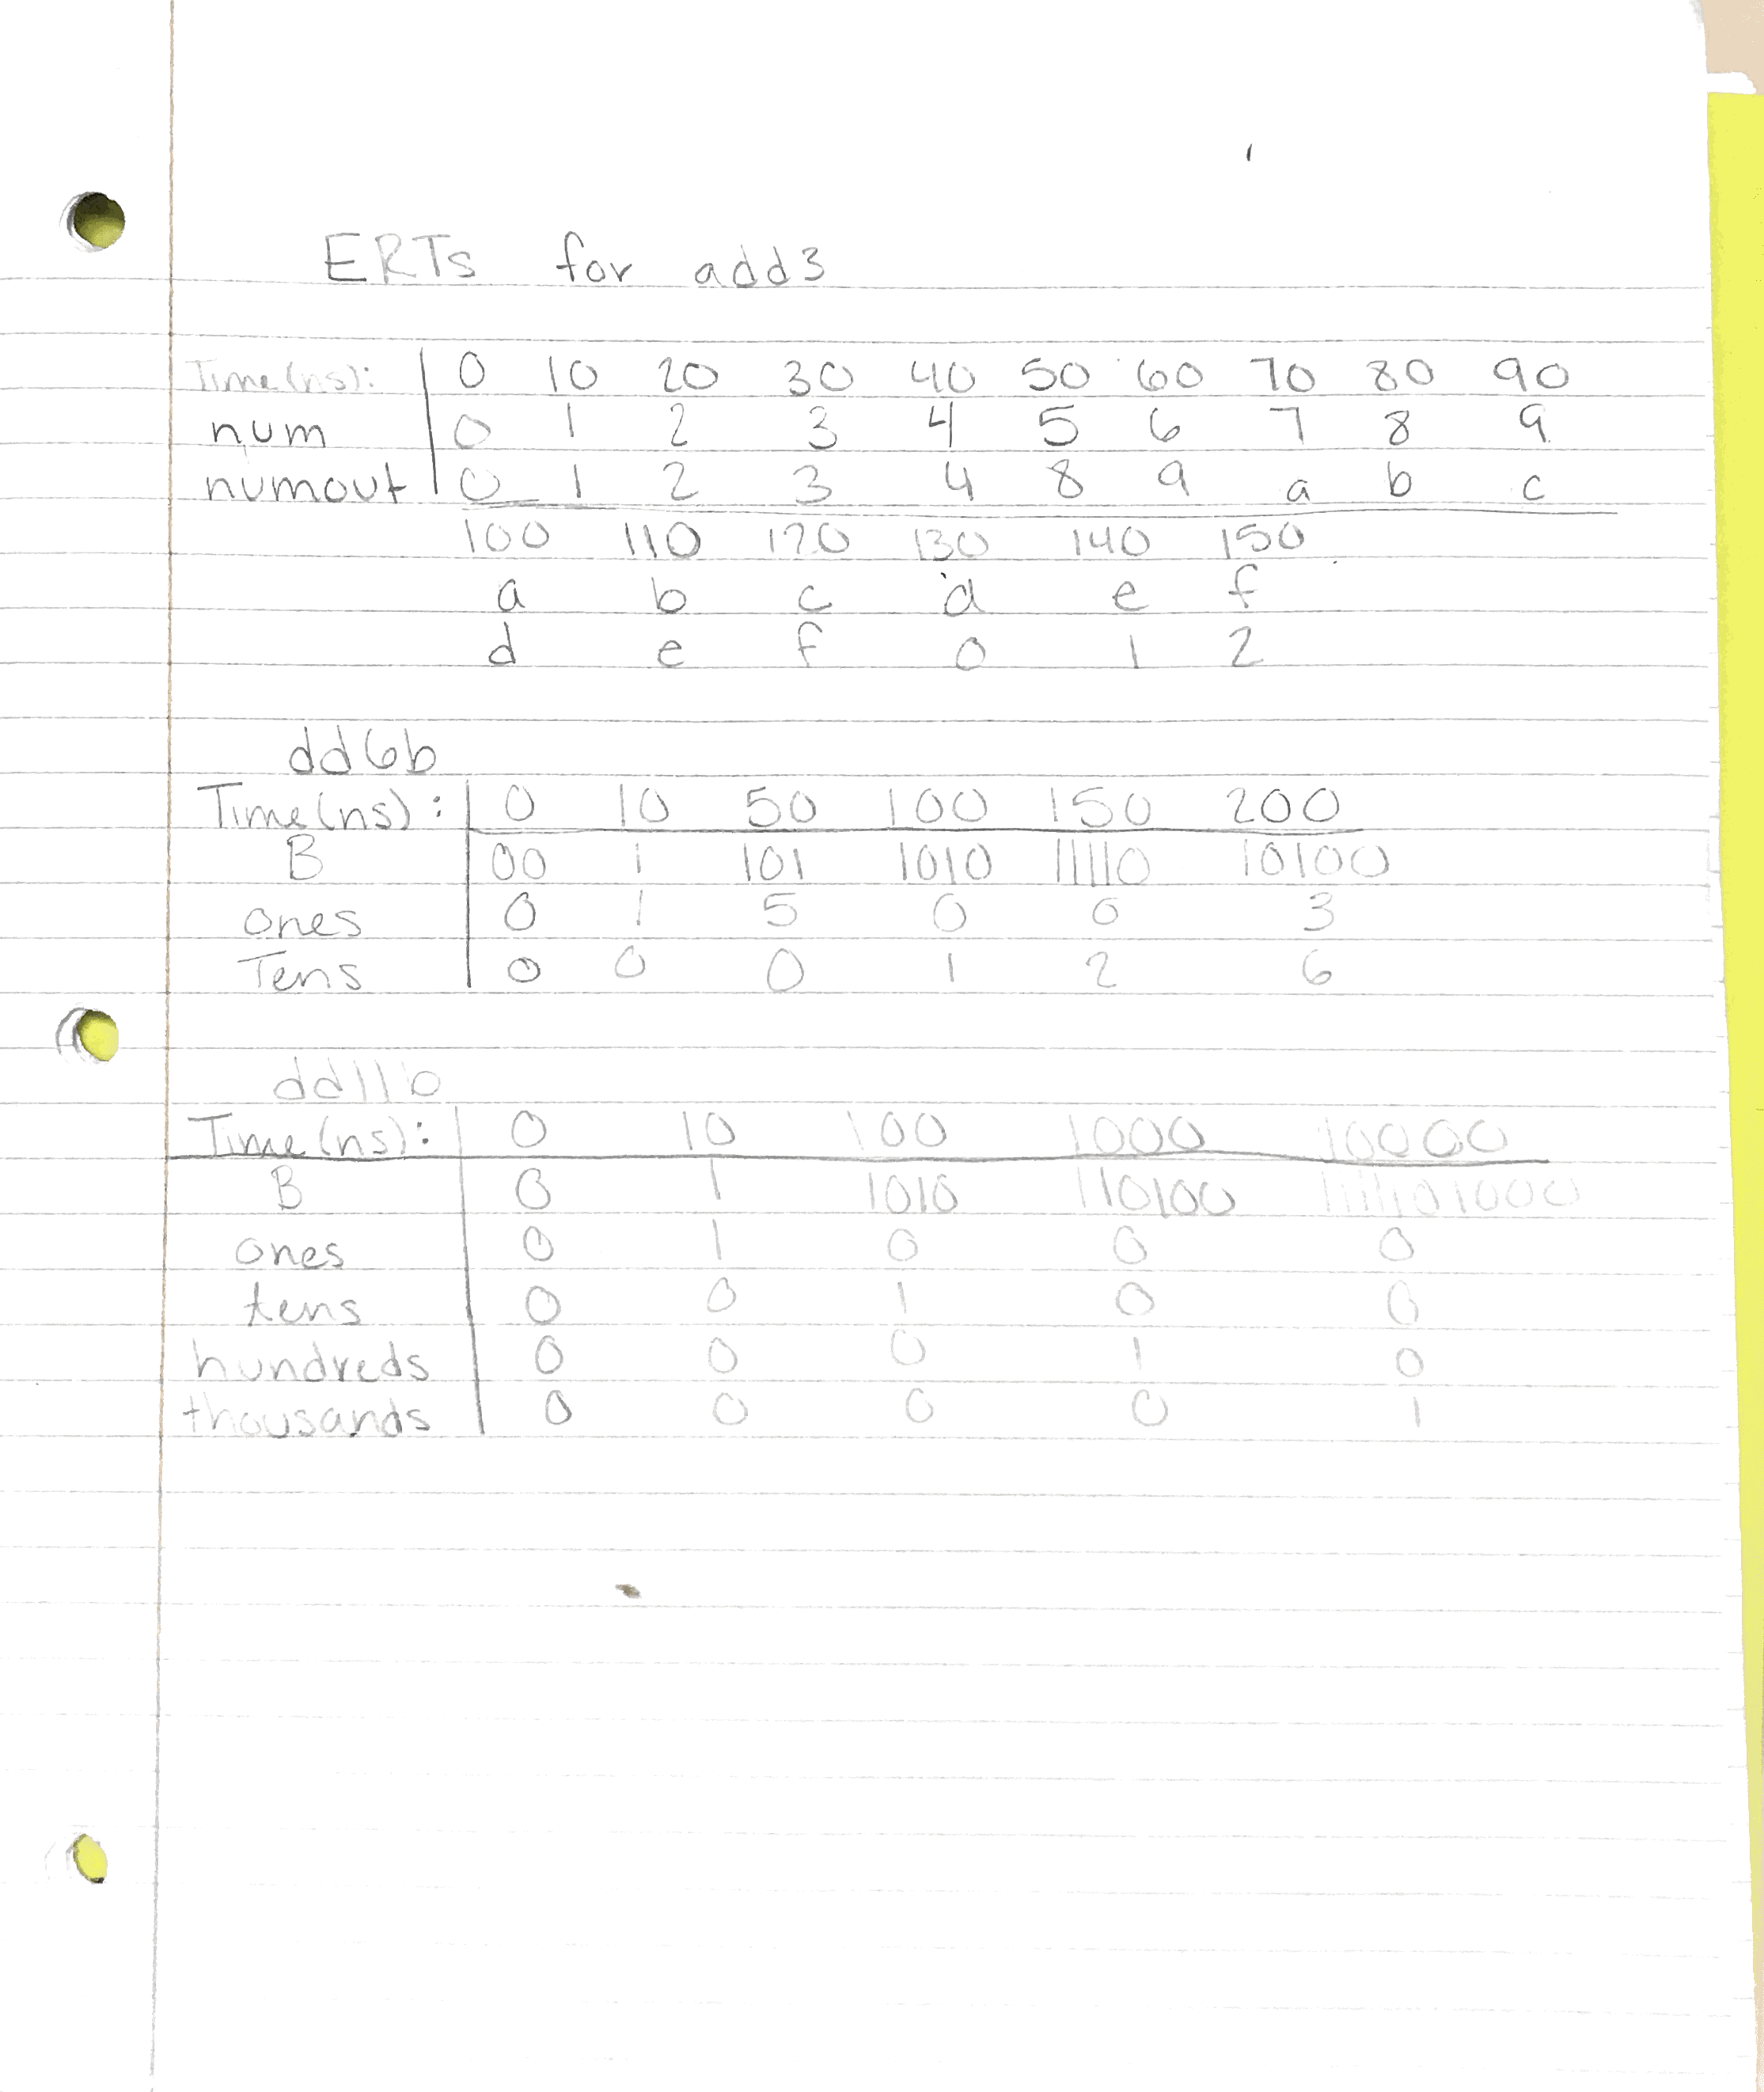
\includegraphics[width= \textwidth]{ERT.png}
	\caption{Estimated Results Table }\label{fig:ERT}
\end{figure}
\begin{figure}
	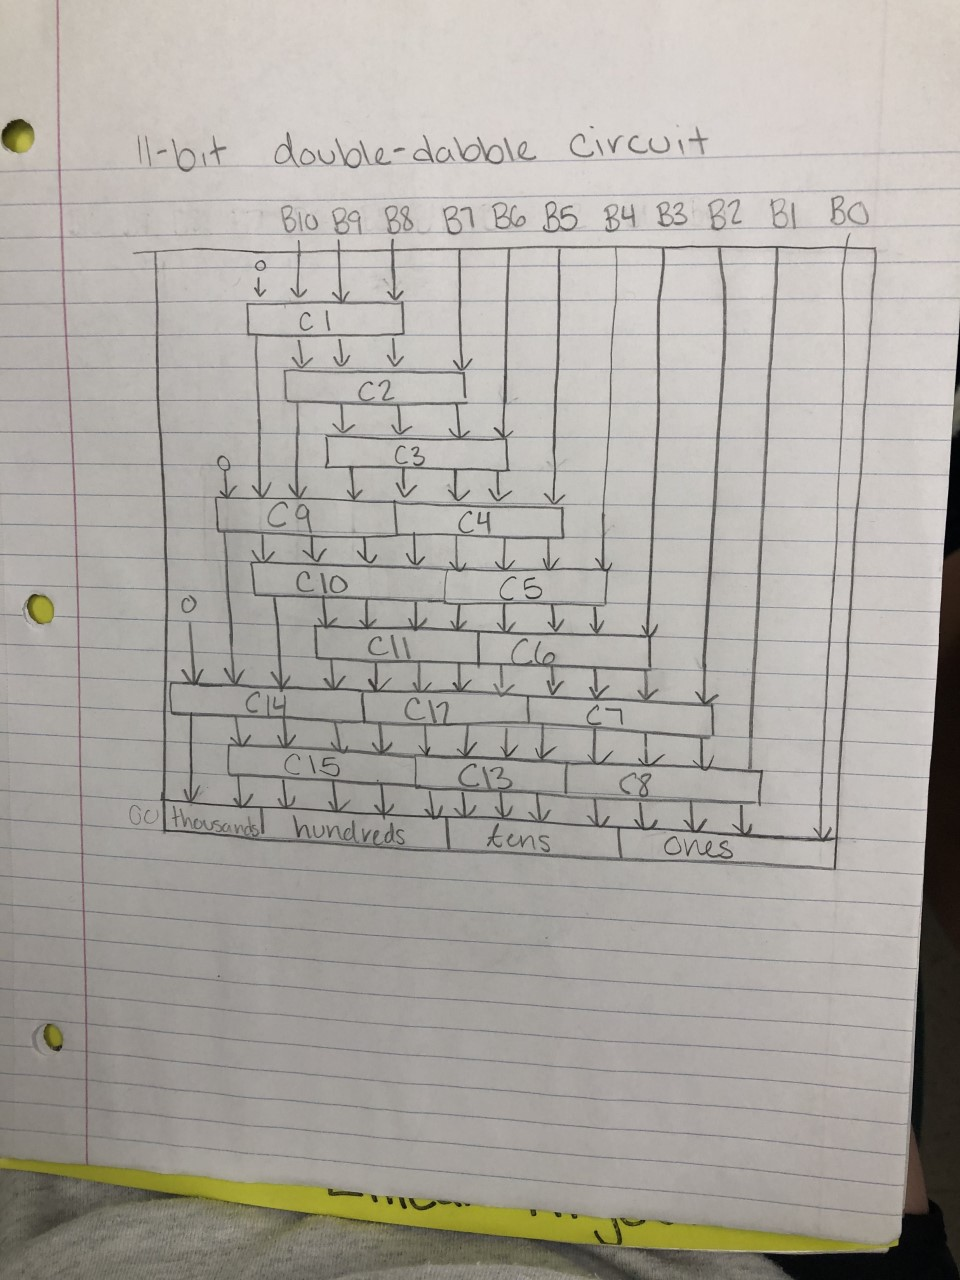
\includegraphics[width= \textwidth]{11-bitcircuit.png}
	\caption{11 bit circuit drawing}\label{fig:11bitcircuit}
\end{figure}\\


\end{document}
